\chapter{Introduction}\label{ch:intro}

\section{Motivation}
\ac{GNSS} receivers should provide accurate and reliable guidance for space vehicles during launch and re-entry. Accurate guidance helps ensure safe, repeatable and cost effective access to space.

However, significant dynamics and vibrations experienced during launch and re-entry prevent \ac{GNSS} receivers from reliably tracking the signal from \ac{GNSS} satellites. This in turn prevents the receiver from providing accurate position, velocity and timing information to the spacecraft, forcing engineers to rely on inferior solutions for guiding the spacecraft. Using a modified version of the \ac{NAMURU} \ac{GNSS} receiver optimised for high dynamics, accurate and reliable performance can be achieved during periods of significant dynamics during launch and re-entry. 

In this thesis, novel modifications to the receiver are analysed for their feasibility and steps for effective implementation are suggested.


In order to understand the value proposition of this thesis to the space industry, it is instructive to examine a specific application. The Falcon 9 V1.1, constructed and launched by
Space Exploration Technologies is a 70m tall, 540
ton, \$85M rocket capable of launching payloads of
up to 4.85 tons to Low Earth Orbit (LEO).
During the ascent, accurate knowledge of the
velocity of the rocket is vital for placing the payload
in the correct orbit. The velocity of the rocket is used
to determine when to shut off the 2nd stage engine,
Every second worth of additional fuel carried for the
engine costs \$1.7M in lost payload revenue, hence
accurately estimating the velocity is crucial. Each
m/s error in velocity changes the orbital height of the
payload by 1.6Km, and requires \$70,000 worth of
fuel to correct.

In order to reduce costs, the body of 1st stage can fly
back to a waiting barge and land, allowing a
significant component of the rocket to be reused.
Safely landing the rocket requires accurate
estimates of position and velocity, with minimal
margin for error. Accurate measurement of velocity
of the 1st stage allows an optimum trajectory to be
planned, optimising the fuel burn and allowing more
cargo, worth \$5,000 a kg to be carried into orbit.

From this, it is possible to conclude that development of a reliable high dynamics GNSS receiver optimised for guiding launcher vehicles is likely to have a significant beneficial effect on the economics of spaceflight.

\section{Problem definition \& project objectives}

The University of New South Wales has been developing the \ac{NAMURU} family of \ac{GNSS} receivers since 2004\cite{MumfordNamuru}. The Namuru family of receivers uses a digital base-band processor implemented on a \ac{FPGA}\cite{Glennon11aquariusfirmware}. A photo of a recent incarnation of the receiver can be seen in figure \ref{fig:Namuru1}.

\begin{figure}[!htb] 
    \centering
    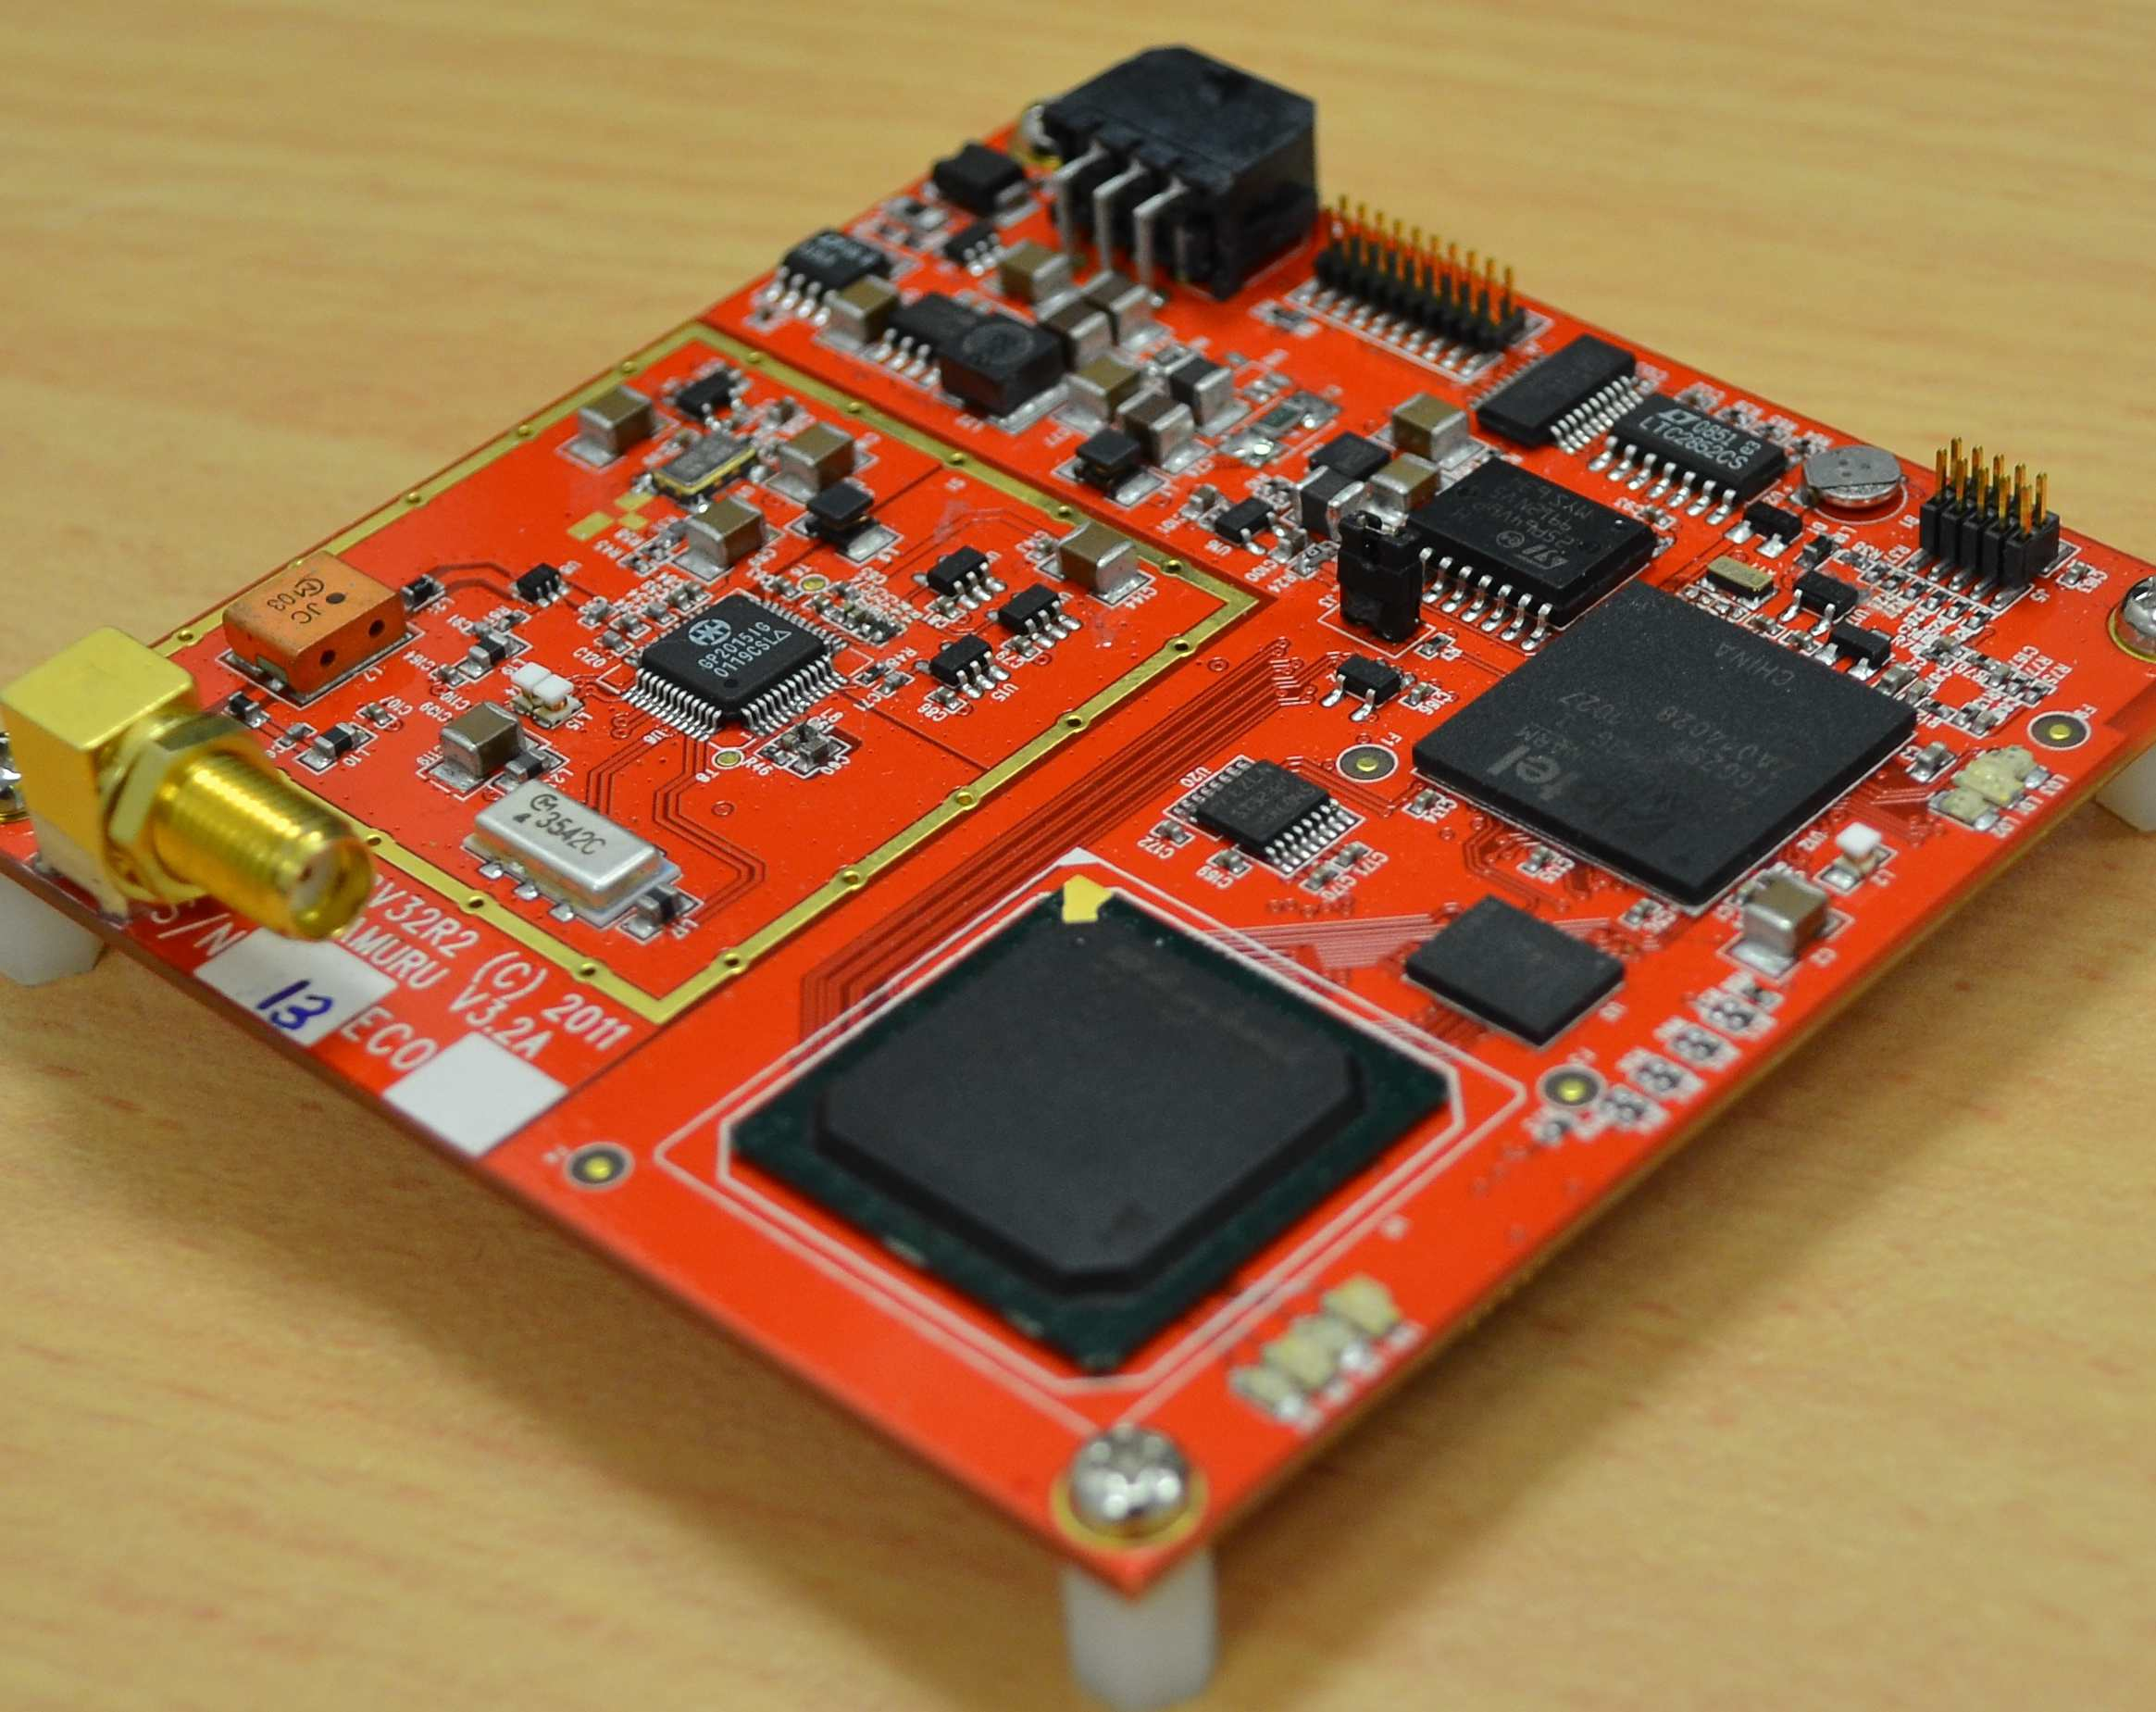
\includegraphics[width=1\textwidth]{Introduction/Namuru1.JPG} 
    \caption{The Namuru V3.2 receiver. The Zarlink GP2015 \ac{RF} front-end on the left of the board is normally covered by a \ac{RF} shield.}
    \label{fig:Namuru1}
\end{figure}

While the operation of the receiver has been validated both on land, and under simulated ballistic spaceflight conditions \cite{NamuruSpaceflight1,NamuruSpaceflight2}, the receiver is currently unable to reliably operate in high dynamics situations. 

In particular, the \ac{PLL} is unable to cope with high dynamics, and looses phase lock. This is because of: 
\begin{itemize}
\item{The doppler shift due to the \ac{LOS} dynamics between the satellite and the \ac{SV}}
\item{The frequency shift in the local oscillator due to the effect of dynamics of the quartz crystal}
\end{itemize}

The aim of this thesis is to improve the high dynamics performance of the \ac{NAMURU} receiver, by investigating the following issues:  

\begin{itemize}
\item{A concrete theoretical understanding of the current implementation}
\item{Validation of the existing implementation against the theory}
\item{Effect of jitter and lag on the \ac{PLL}}
\item{Alternative lock detectors and switching logic}
\item{Implementing new techniques discussed in the literature}
\item{Effects of vibration on the \ac{PLL}}
\end{itemize}

The objectives of this thesis are as follows : 
\begin{itemize}
\item{Sustained tracking with \ac{LOS} dynamics of 15 g \& jerks of 10g/s.}
\item{Reliable operation during simulations of launch and re-entry}
\item{Reliable operation while while experiencing realistic levels of vibration}
\end{itemize}

